\documentclass{standalone}

\usepackage[OT1]{fontenc}
\renewcommand*\familydefault{\sfdefault}
\usepackage{helvet,sfmath}
\usepackage{siunitx}

\usepackage{tikz}
\usetikzlibrary{arrows,calc,patterns}
% \usetikzlibrary{intersections, calc, arrows.meta}
\usepackage{tikz,tkz-euclide}

\definecolor{square}{RGB}{177,162,202}

\begin{document}

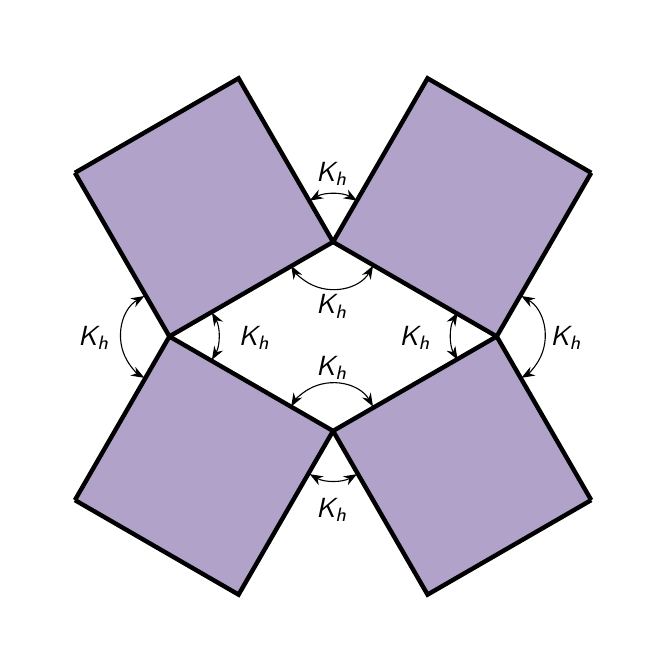
\begin{tikzpicture}[scale=0.6]
    %% Background
    \draw[draw=none] (-1,-1) to (-1,1) to (12,12) to (12,-1) to (-1,-1);
    %% Auxetic structure
    \foreach \angle in {60}
    {
        \foreach \x in {1}
        {
            \foreach \y in {1}
            {
                \draw[ultra thick, fill=square] 
                ( 0, {4*\y*sin(\angle/2)} )
                to ( {4*\x*sin(\angle/2)}, {4*\y*sin(\angle/2) + 4*\y*cos(\angle/2)} )
                to ( {4*\x*sin(\angle/2) + 4*\x*cos(\angle/2)}, {4*\y*cos(\angle/2)} )
                to ( {4*\x*cos(\angle/2)}, 0)
                to ( 0, {4*\y*sin(\angle/2)} )
                ;
                \draw[ultra thick, fill=square] 
                ( 0, {4*\y*sin(\angle/2) + 2*4*\y*cos(\angle/2) } )
                to ( {4*\x*sin(\angle/2)}, {4*\y*sin(\angle/2) + 4*\y*cos(\angle/2)} )
                to ( {4*\x*sin(\angle/2) + 4*\x*cos(\angle/2)}, {2*4*\y*sin(\angle/2) + 4*\y*cos(\angle/2)} )
                to ( {4*\x*cos(\angle/2)}, {2*4*\y*sin(\angle/2) + 2*4*\y*cos(\angle/2)})
                to ( 0, {4*\y*sin(\angle/2) + 2*4*\y*cos(\angle/2)} )
                ;
                \draw[ultra thick, fill=square] 
                ( {2*4*\x*sin(\angle/2) + 2*4*\x*cos(\angle/2)}, {4*\y*sin(\angle/2)} )
                to ( {4*\x*sin(\angle/2) + 2*4*\x*cos(\angle/2)}, {4*\y*sin(\angle/2) + 4*\y*cos(\angle/2)} )
                to ( {4*\x*sin(\angle/2) + 4*\x*cos(\angle/2)}, {4*\y*cos(\angle/2)} )
                to ( {2*4*\x*sin(\angle/2) + 4*\x*cos(\angle/2)}, 0)
                to ( {2*4*\x*sin(\angle/2) + 2*4*\x*cos(\angle/2)}, {4*\y*sin(\angle/2)} )
                ;
                \draw[ultra thick, fill=square] 
                ( {2*4*\x*sin(\angle/2) + 2*4*\x*cos(\angle/2)}, {4*\y*sin(\angle/2) + 2*4*\y*cos(\angle/2)} )
                to ( {4*\x*sin(\angle/2) + 2*4*\x*cos(\angle/2)}, {4*\y*sin(\angle/2) + 4*\y*cos(\angle/2)} )
                to ( {4*\x*sin(\angle/2) + 4*\x*cos(\angle/2)}, {2*4*\y*sin(\angle/2) + 4*\y*cos(\angle/2)} )
                to ( {2*4*\x*sin(\angle/2) + 4*\x*cos(\angle/2)}, {2*4*\y*sin(\angle/2) + 2*4*\y*cos(\angle/2)})
                to ( {2*4*\x*sin(\angle/2) + 2*4*\x*cos(\angle/2)}, {4*\y*sin(\angle/2) + 2*4*\y*cos(\angle/2)} )
                ;
            }
        }
    }
    %% Stiffness
    \draw[Stealth-Stealth] (2.9,5.97) arc(30:-30:1);
    \draw[Stealth-Stealth] (8.1,5.97) arc(150:210:1);
    \draw[Stealth-Stealth] (1.47,6.32) arc(120:240:1);
    \draw[Stealth-Stealth] (9.45,6.32) arc(60:-60:1);
    \draw[Stealth-Stealth] (5.97,8.34) arc(60:120:1);
    \draw[Stealth-Stealth] (5.97,2.55) arc(300:240:1);
    \draw[Stealth-Stealth] (6.31,3.98) arc(30:150:1);
    \draw[Stealth-Stealth] (6.31,6.96) arc(330:210:1);
    \draw
    (0.4,5.44) node{\(K_h\)}
    (3.8,5.44) node{\(K_h\)}
    (7.2,5.44) node{\(K_h\)}
    (10.4,5.44) node{\(K_h\)}
    (5.44,1.8) node{\(K_h\)}
    (5.44,4.8) node{\(K_h\)}
    (5.44,6.1) node{\(K_h\)}
    (5.44,8.9) node{\(K_h\)}
    ;
\end{tikzpicture}

\end{document}
